%-\textbf{}%\documentclass[a4paper,12pt]{upthesis}
\documentclass[a4paper,12pt]{upthesis}

\usepackage{graphicx}
\usepackage{amsmath}
\usepackage{amssymb}
%\usepackage{natbib}
% แพคเกจสำหรับสร้าง hyperlink ด้วยคำสั่ง \href{<url>}{<Text to show>}
%\usepackage[linktocpage=true]{hyperref}       % Create hyperlink with command \href{<url>}{<Text to show>}.

% แพคเกจสำหรับเรียกใช้การหมุนภาพ หรือตาราง
\usepackage{rotating}       % Package for rotating either figure or table with command
                                      %\begin{sidewaysfigure} or \begin{sidewaystable} and also \end{} as well.
\usepackage{enumitem}		% For customize the symbols or enumeration                                      

% เป็นการกำหนดค่าเลขหน้าภาษาไทยในช่วงแรก
\usepackage{polyglossia}
\setdefaultlanguage{thai}
\setotherlanguages{thai}
% เป็นการกำหนดแพคเกจสำหรับจัดการเรื่องฟอนต์ รวมถึงการใช้ภาษาไทย
\usepackage{fontspec}
\usepackage{xunicode}
\usepackage{xltxtra}

\usepackage{indentfirst}
\usepackage{fancybox}
\usepackage{pst-grad}
\usepackage{pst-osci}
\usepackage{pst-coil}
\usepackage{tabularx}

\usepackage[labelfont=bf, textfont=bf]{caption}
\usepackage{floatrow}
\floatsetup[table]{style=plaintop, footnoterule=none,footskip=.35\skip\footins}  

% กำหนดการตัดคำ ขนาด และฟอนต์ที่จะใช้สำหรับภาษาไทย
\XeTeXlinebreaklocale "th_TH"
\XeTeXlinebreakskip = 0pt plus 1pt
\defaultfontfeatures{Scale=1.23}
\setmainfont[Mapping=tex-text]{TH Sarabun New}

%\setdefaultlanguage{thai}
%\newfontfamily{\thaifont}[Script=thai]{TH Niramit AS}

\usepackage{pstricks,pst-plot,pst-node}
\usepackage{pst-3dplot}
\usepackage{pstricks-add}

\usepackage{makeidx}         % allows index generation
\usepackage{graphicx}        % standard LaTeX graphics tool
                                             % when including figure files
\usepackage{multicol}         % used for the two-column index
\usepackage[bottom]{footmisc}% places footnotes at page bottom
\usepackage{tensor}             %for write tensor indices
\usepackage{color}                 % for assign a color to text with command
                                        %\textcolor{color}{text}
\usepackage{enumitem}		% For customize the symbols or enumeration                           

%Package for setup page (paper size)
% สำหรับการกำหนดขนาดของกระดาษ   *** แก้ไขได้ หากใช้กระดาษ และจัดขอบกระดาษต่างจากนี้ ***
\usepackage{geometry}
 \geometry{
 a4paper,		% Paper size ขนาดกระดาษ
 total={147.5mm,234.5mm},	% Total area of text on the page	ขนาดกว้างยาวของพื้นที่สำหรับข้อความในกระดาษ
 left=37.5mm,			% Left margin	1 inch = 25.4 mm ระยะขอบซ้าย
 %right=25mm,				% Right margin ระยะขอบขวา (ไม่กำหนดก็ได้ เพราะจะจัดอัตโนมัติ)
 top=37.5mm,			% Top margin	1.5 inch = 38.1 mm ระยะขอบบน
% bottom=25mm,		% Bottom margin ระยะขอบล่าง (ไม่กำหนดก็ได้ เพราะจะจัดอัตโนมัติ)
 }


% การนิยามคำสั่งที่ใช้บ่อย และยาว ให้สั้นลง
\def\l{\left}
\def\r{\right}
%\def\be{\begin{equation}}
%\def\ee{\end{equation}}
%\def\bea{\begin{eqnarray}}
%\def\eea{\end{eqnarray}}
\def\f{\frac}
\def\no{\nonumber}
\def\i{\hat{i}}
\def\j{\hat{j}}
\def\k{\hat{k}}
\def\ro{\hat{\rho}}
\def\vp{\hat{\varphi}}
\def\x{\hat{x}}
\def\y{\hat{y}}
\def\z{\hat{z}}
\def\e#1{\hat{e}_{#1}}
\def\rh{\hat{r}}
\def\tt{\hat{\theta}}
\def\ph{\hat{\phi}}
\def\cross{\times}
\def\pd{\partial}
\def\pdx{\frac{\partial}{\partial x}}
\def\pdy{\frac{\partial}{\partial y}}
\def\pdz{\frac{\partial}{\partial z}}
\def\pdt{\frac{\partial}{\partial t}}
\def\ddx{\frac{d}{dx}}
\def\ddy{\frac{d}{dy}}
\def\ddz{\frac{d}{dz}}
\def\ddt{\frac{d}{dt}}
\def\pt#1#2{\frac{\partial{#1}}{\partial{#2}}}
\def\dd#1#2{\frac{d{#1}}{d{#2}}}
\def\det#1{\rm det({#1})}
\def\tr#1{\rm Tr({#1})}
\def\ul#1{\rm \underline{#1}}
\def\dul#1{\rm \underline{\underline{#1}}}
\def\mi#1#2{\rm M_{#1}(\underline{#2})}
\def\co#1#2{\rm C_{#1}(\underline{#2})}
\def\red#1{\textcolor{red}{#1}}
\def\blue#1{\textcolor{blue}{#1}}
\def\w9{{\rm WMAP9+BAO+}$H_0$}
\def\p15{$TT,TE,EE${\rm +lowP+Lensing+ext}}


% More references in gloss-thai of polyglossia package
% http://texdoc.net/texmf-dist/tex/latex/polyglossia/gloss-thai.ldf
% \thaiAlpha works well, the sequence is ก ข "ฃ" ค "ฅ" ฆ ง จ ...
% Normally, we need ก ข ค ง จ which is defined in \thaialph
% I'm not sure why it doesn't work. So, I just re-define it.
\def\thaialph#1{\expandafter\thalph\csname c@#1\endcsname}
\def\thalph#1{%
    \ifcase#1\or ก\or ข\or ค\or ง\or จ\or ฉ\or ช\or ซ\or
    ฌ\or ญ\or ฎ\or ฏ\or ฐ\or ฑ\or ฒ\or ณ\or ด\or ต\or ถ\or ท\or ธ\or น\or
    บ\or ป\or ผ\or ฝ\or พ\or ฟ\or ภ\or ม\or ย\or ร\or ฤ\or ล\or ฦ\or ว\or
    ศ\or ษ\or ส\or ห\or ฬ\or อ\else ฮ\else\xpg@ill@value{#1}{thalph}\fi}

\usepackage{subcaption}
%\renewcommand{\figurename}{รูปที่}
% กำหนดให้ subfigurename เป็น (ก), (ข), (ค), ...
\renewcommand{\thesubfigure}{\thaialph{subfigure}}	


\usepackage{array,tabularx}
\makeatletter
\def\thline#1{%
    \noalign {\ifnum 0=`}\fi \hrule height #1
    \futurelet \reserved@a \@xhline
}
\def\tvline#1{@{\hskip\tabcolsep\vrule width #1\hskip\tabcolsep}}
\makeatother
% End of make thick hline and vline

% package{multirow} ใช้รวมแถวในตาราง
%package{multirow} is use to combine the rows in a table.
\usepackage{multirow}
% package{array} ใช้ขยายความสูงของแต่ละแถวในตาราง
%package{array} is use to expand the height of each row in a table.
\usepackage{array}
\title{  						% Title in Thai ชื่อเรื่องภาษาไทย
พลังงานมืดแบบกฎกำลังของเตคีออน
}
\titleen{						% Title in English ชื่อเรื่องภาษาอังกฤษ
Tachyonic Power-Law Dark Energy
}

% คำนำหน้าผู้เขียน
\nameprefix{นางสาว}
\nameprefixen{Miss}

% ชื่อ และนามสกุลของผู้เขียน
% \author{Name}{Surname}
\author{น้ำเพชร}{แก้ววิลัย}
\authoren{Nampetch}{Kaewwilai}


% your figure ใส่ไฟล์รูปของผู้เขียน
\myfig{CylinderCoor.png}

% ชื่ออาจารย์ที่ปรึกษา
\advisor{ดร.พงศพัศ แรงดี}                                % advisor
\advisoren{Dr.Phongsaphat Rangdee}

% ชื่ออาจารย์ที่ปรึกษาร่วม
\coadvisor{ดร.ชลธิชา กฤษณ์เพ็ชร}
\coadvisoren{Dr.Chonticha Kritpetch}

%ชื่อปริญญา
\degree{วิทยาศาสตรบัณฑิต}                                   % degree
\degreeen{Bachelor of Science}
%ชื่อย่อปริญญา
\degreeAbb{วท.บ.}                                               % degree (abbreviation)
\degreeAbben{B.Sc.}

%หลักสูตร หรือสาขาวิชา
\major{ฟิสิกส์}                                      % major
\majoren{Physics}

% ภาควิชา หรือสาขาวิชา
\dept{ภาควิชาฟิสิกส์}                      % department

% เดือน และปี พ.ศ. ที่สำเร็จการศึกษา
\date{ตุลาคม 2565}                                               % date

% ปีการศึกษา
\academicyear{2565}                                             % academic year

% คำสำคัญ ภาษาไทย  และภาษาอังกฤษ
\keywordsth{                                                      % keywords in Thai คำสำคัญ ภาษาไทย ควรมีแค่ 3-4 คำ
            แก๊สแชปลีจิน, พลังงานมืด, สนามสเกลาร์, เอกภพที่เร่งออก
         }
\keywords{						% Keywords in English คำสำคัญ ภาษาอังกฤษ ไม่ควรยาวมาก และควรมีแค่ 3-4 คำ
			Chaplygin Gas, Dark Energy, Accelerating Universe, Phantom Power-Law
		}

% your working place สถานที่ทำงาน (ถ้ามี)
%\workplace{}
%\position{Lecturer at University of Phayao}
%\workplace{Department of Physics, Faculty of Science, University of Phayao, Phayao 56000, Thailand}

% Work Experiences ประสบการณ์การทำงาน (ถ้ามี)
%\WorkExpr{      
%\workexpr{2005 - 2009}{Lecturer at Department of Physics, Faculty of Science, University of Phayao, Phayao, Thailand}
%\workexpr{2000 - 2001}{Lecturer at Department of Physics, Faculty of Science, Naresuan University, Phitsanulok, Thailand}
%}
%Publication List  รายการผลงานตีพิมพ์ (ถ้ามี)
%\Publication{   
%\publication{1}{\textbf{Rachan Rangdee} (IF) and Burin Gumjudpai (IF and ThEP), ``Tachyonic (phantom) power-law cosmology'', Astrophysics and Space Science \textbf{349} (2014) 975-984.
%[arXiv:1210.5550 [astro-ph.CO]]}
%\publication{2}{Burin Gumjudpai (IF and ICTP) and \textbf{Phongsaphat Rangdee} (IF), ``Non-minimal derivative coupling gravity in cosmology'', General Relativity and Gravitation \textbf{47} (2015) 140.
%[arXiv:1511.00491 [gr-qc]]}
%}

% Oral and Poster Presentation List  รายการการนำเสนอทั้งแบบ Oral & Poster
%\Presentation{          
%\presentation{1}{\textbf{Rachan Rangdee} and Burin Gumjudpai (IF), ORAL ``Non-minimal Derivative Coupling with Power-Law'', RGJ-Ph.D. Congress XVI ``ASEAN: Emerging Research Oppotunities'', Pattaya, Chonburi, Thailand (2015).}
%\presentation{2}{\textbf{Rachan Rangdee} (IF), ORAL ``Aspects of non-minimal derivative coupling'', the $7^{\rm th}$ Aegean Summer School Beyond Einstein's Theory of Gravity, Parikia, Island of Paros, Greece, (2013).}
%\presentation{3}{\textbf{Rachan Rangdee} (IF), ORAL ``Tachyonic Phantom Power-Law Cosmology'', the Workshop on Heavy Ion and High Energy Physics 2012 (HIHEP2012), Naresuan University, Phitsanulok, Thailand (2012).}
%\presentation{4}{\textbf{Rachan Rangdee} (IF), ORAL ``Tachyonic Power-Law Cosmology'', the Siam Physics Congress 2012 (SPC2012): Past, Present and Future of Physics, Phranakhon Si Ayutthaya, Thailand (2012).}
%\presentation{5}{\textbf{Rachan Rangdee} (TPTP), POSTER ``TACHYONIC DARK ENERGY MODEL: DYNAMICS AND EVOLUTION'', the $11^{\rm th}$ Asian-Pacific Regional IAU Meeting (APRIM2011), Chiang Mai, Thailand (2011).}
%}

%%%%%%%%%%%%%%%%%%%%%%%%%%%%%%%%%%%%%%%%%%%%%%%%%%%%%%%%%%%%%%%%%%%%%%
%%%  เริ่มต้นเอกสาร
%%%%%%%%%%%%%%%%%%%%%%%%%%%%%%%%%%%%%%%%%%%%%%%%%%%%%%%%%%%%%%%%%%%%%%

\begin{document}

\pagenumbering{thaialph}
%\maketitle
%\newpage
%%%%%%%%%%%%%%%%%%%%%%%%%%%
%%%
%%% MAKE A COVER PAGE
%%% สร้างหน้าปก (หน้าแรก)
%%%%%%%%%%%%%%%%%%%%%%%%%%%%%

\thispagestyle{empty}
\begin{center}
  \Large{\textbf{Windows Server 2022\\}}
  \vspace{3cm}
  \centering
  \begin{center}
  \textbf{จัดทำโดย\\}
  \vspace{1cm}
  นายก้องนภา\hspace{0.6cm}วังตา \hspace{1cm} รหัสนิสิต \hspace{0.2cm} 64020529\\
  นายปฏิวัติ\hspace{1.1cm}จำศิล \hspace{0.9cm} รหัสนิสิต \hspace{0.2cm} 64020675\\
  นายสพลดนัย\hspace{0.5cm}พรหมศรี \hspace{0.25cm} รหัสนิสิต \hspace{0.2cm} 64020811\\
  นายสิรวิชญ์\hspace{0.9cm}คำชุ่ม \hspace{0.85cm} รหัสนิสิต \hspace{0.2cm} 64020822\\
  นายสุริยา\hspace{1.3cm}หาญจริง \hspace{0.3cm} รหัสนิสิต \hspace{0.2cm} 64020833\\
  นายจิรศักดิ์\hspace{1cm}อุ่นบ้าน \hspace{0.45cm} รหัสนิสิต \hspace{0.2cm} 64024309\\
  \end{center}
  \vspace{3cm}
  \textbf{เสนอ\\}
  อาจารย์วรกฤต แสนโภชน์\\

  \vspace{4cm}
  \textbf{สาขาวิทยาการคอมพิวเตอร์   คณะเทคโนโลยีสารสนเทศและการสื่อสาร\\
  รายวิชา 225331[2] แนวคิดระบบปฎิบัติการ\\
  ภาคเรียนที่ 2 ปีการศึกษา 2566\\}
  \end{center}
  
  

%%%%%%%%%%%%%%%%%%%%%%%%%%%%%%%%%%%%%%%%%%%%%%%%%%%%%%%%%%%%%%%%%%%%%%%
% กำหนดเลขหน้าเป็นเลขอารบิ
\pagenumbering{arabic}
\pagestyle{headings}
\setcounter{page}{1}

\newpage

%%%%%%%%%%%%%%%%%%%%%%%%%%%%%
%%%
%%% ADD CHAPTER TO THE MAIN FILE เพิ่มเนื้อหาของแต่ละบท
%%%
%%%%%%%%%%%%%%%%%%%%%%%%%%%%%

\baselineskip=8mm
\renewcommand{\thesection}{\arabic{section}.}
\renewcommand{\theequation}{\thesection.\arabic{equation}}
\numberwithin{equation}{section}
\renewcommand{\thesection}{}
\renewcommand{\thesubsection}{}
\renewcommand{\thesubsubsection}{\thesubsection\arabic{subsubsection}.}
\renewcommand{\caption}{}

\section{ประวัติความเป็นมา}

Windows Server คือ ระบบปฏิบัติการที่ออกแบบโดย Microsoft ซึ่ง Windows Server สนับสนุนการจัดการระดับองค์กรการจัดเก็บข้อมูลแอพพลิเคชันและการติดต่อสื่อสาร Windows Server มีความสำคัญต่อเสถียรภาพความปลอดภัยระบบเครือข่ายและการปรับปรุงระบบไฟล์ต่างๆ การปรับปรุงอื่น ๆ รวมถึงการปรับปรุงเทคโนโลยีการติดตั้งรวมถึงการสนับสนุนฮาร์ดแวร์ที่เพิ่มขึ้น \cite{ประวัติความเป็นมา:1}
ออกแบบมาเพื่อให้ใช้งานเฉพาะทาง กับเครื่อง Super Computer หรือ เครื่อง Server ที่มีการประมวลข้อมูลพร้อม ๆ กันจำนวนมหาศาล รองรับการเข้าใช้งาน หรือเข้าถึงข้อมูลพร้อมกันหลาย ๆ คนได้ อย่างเช่น Web Server, File Server, Data Center Server, Mail Server เป็นต้น \cite{ประวัติความเป็นมา:2}
โดยพัฒนาการของ Windows Server มีลำดับดังนี้ \cite{ประวัติความเป็นมา:Windows Server}

\hspace{0cm}\subsection{1993 : Windows NT 3.1 Advanced Server Microsoft :}มีการเปิดตัวระบบปฏิบัติการ Windows NT ในสองรูปแบบ รูปแบบหนึ่งสำหรับเวิร์กสเตชันและอีกรูปแบบสำหรับเซิร์ฟเวอร์ ระบบปฏิบัติการ 32 บิตมีฮาร์ดแวร์ abstraction layer (HAL) ซึ่งให้ความเสถียรของระบบมากขึ้นโดยการบล็อกแอปพลิเคชันไม่ให้เข้าถึงฮาร์ดแวร์ระบบโดยตรง บริษัทต่างๆสามารถใช้เซิร์ฟเวอร์ขั้นสูงเป็นตัวควบคุมโดเมนเพื่อจัดเก็บสิทธิ์ของผู้ใช้และกลุ่มได้

\hspace{0cm}\subsection{1994: Windows NT 3.5 Server :}มีการอัปเดตคุณลักษณะเครือข่ายหลักในเซิร์ฟเวอร์รุ่นนี้และเพิ่มการสนับสนุนแบบรวมสำหรับ TCP/IP และ Winsock การปรับปรุงเครือข่ายอื่นๆ อนุญาตให้ผู้ใช้บนระบบปฏิบัติการอื่นๆ ที่ไม่ใช่ Microsoft สามารถเข้าถึงไฟล์และแอปพลิเคชันบนโดเมนได้ 

\hspace{0cm}\subsection{1995: Windows NT Server 3.51 :}มีการปรับแต่งรุ่นนี้เพื่อเพิ่มประสิทธิภาพและลดจำนวนหน่วยความจำ ระบบปฏิบัติการเซิร์ฟเวอร์นี้ได้รับการปรับให้เหมาะสมเพื่อให้บริการแก่ผู้ใช้ได้เร็วขึ้นผ่านการอัปเดตเครือข่ายและการใช้สแต็ก มีการสนับสนุนการเชื่อมต่อเพิ่มเติมสำหรับบริษัทในสภาพแวดล้อมแบบผสมกับเซิร์ฟเวอร์ Windows NT และ NetWare เพื่อให้ผู้ใช้สามารถรับบริการจากแต่ละแห่งด้วยข้อมูลประจำตัว TCP/IP และ Winsock 

\hspace{0cm}\subsection{1996: Windows NT Server 4.0 :}มีการยืมอินเทอร์เฟซมาจาก Windows 95 และยังใช้แอปพลิเคชันจำนวนมากในระบบปฏิบัติการไคลเอ็นต์ เช่น File Explorer มีการขยายขีดความสามารถของโปรโตคอลเครือข่าย เพื่อให้ทรัพยากรเครือข่ายพร้อมใช้งานสำหรับเครื่องที่ไม่ใช่ของ Microsoft ในวงกว้างขึ้น คุณลักษณะหลักในเวอร์ชั่นนี้คือความสามารถในการใช้เซิร์ฟเวอร์เป็นเซิร์ฟเวอร์ข้อมูลทางอินเทอร์เน็ต ซึ่งปัจจุบันเรียกว่าบริการข้อมูลทางอินเทอร์เน็ต (IIS) และ เซิร์ฟเวอร์ระบบชื่อโดเมน สามารถแนะนำผู้ดูแลระบบผ่านงานต่างๆได้ เช่น การแชร์ฮาร์ดดิสก์ด้วยคุณสมบัติที่เรียกว่า Administrative Wizards ได้รับการปรับให้เหมาะสมเพื่อให้บริการแก่ผู้ใช้ได้เร็วขึ้น

\hspace{0cm}\subsection{2000: Windows 2000 :}มีการเปิดตัว Active Directory ซึ่งเป็นบริการไดเร็กทอรีที่จัดเก็บและจัดการข้อมูลเกี่ยวกับออบเจ็กต์เครือข่าย รวมถึงข้อมูลผู้ใช้ ระบบ และบริการ Active Directory ช่วยให้ผู้ดูแลระบบทำงานต่างๆได้ เช่น การกำหนดค่าเครือข่ายส่วนตัวเสมือนการเข้ารหัสข้อมูล การอนุญาตให้เข้าถึงไฟล์ร่วมกันบนคอมพิวเตอร์ในเครือข่าย คอนโซลการจัดการของ Microsoft (MMC) ระบบไฟล์ NTFS 3.0 และ รองรับไดรฟ์ข้อมูลดิสก์แบบไดนามิก โดย Windows 2000 มีสามรุ่น ได้แก่ Server , Advanced Server และ Datacenter ซึ่งสร้างขึ้นเพื่อทำงานร่วมกับ Windows 2000 Professional ซึ่งเป็นระบบปฏิบัติการไคลเอ็นต์  

\hspace{0cm}\subsection{2003: Windows Server 2003 :}มีการเปิดตัว Windows Server 2003 และมีการปรับปรุงความปลอดภัยให้ดียิ่งขึ้น ได้ปรับแต่งและเพิ่มความปลอดภัยให้กับ IIS ซึ่งเป็นคุณลักษณะของเว็บเซิร์ฟเวอร์ และปิดใช้งานบริการและคุณสมบัครที่ไม่จำเป็น เซิร์ฟเวอร์ในรุ่นนี้อนุญาตให้ผู้ดูแลระบบกำหนดฟังก์ชันเฉพาะให้กับเซิร์ฟเวอร์ เช่น ตัวควบคุมโดเมนหรือเซิร์ฟเวอร์ DNS   ฟังก์ชันการเข้ารหัส ที่ขยายมากขึ้น ไฟร์วอลล์  ในตัว  การรองรับ Network Address Translation (NAT) ที่ดียิ่งขึ้นและบริการ Volume Shadow Copy และในเวอร์ชันนี้ Windows Server 2003 มีสี่รุ่นคือ Standard, Enterprise, Datacenter และ Web 

\hspace{0cm}\subsection{2005: Windows Server 2003 R2 :}การกำหนดชื่อ Microsoft เริ่มใช้การกำหนด R2 หรือรุ่นสองกับ Windows Server 2003 R2 โดยองค์กรจำเป็นต้องซื้อใบอนุญาต Windows Server ใหม่เสมอเพื่อใช้ระบบปฏิบัติการเซิร์ฟเวอร์ใหม่ แต่รุ่น R2 จะใช้ใบอนุญาตการเข้าถึงไคลเอ็นต์ ( CAL ) ของเซิร์ฟเวอร์เวอร์ชันก่อนหน้าได้เพื่อจะไม่ต้องความจำเป็นในการอัพเกรดใบอนุญาตเหล่านั้น เวอร์ชันนี้ได้รับการปรับปรุงเกี่ยวกับคุณลักษณะด้านความปลอดภัยและความปลอดภัยใน Windows Server 2003 คุณสมบัติใหม่ที่สำคัญในรุ่นนี้ได้แก่ \textbf{Active Directory Federation Services }ซึ่งช่วยให้ผู้ดูแลระบบขยายการเข้าถึงแอปพลิเคชันและระบบ การลงชื่อเพียงครั้งเดียวนอกเหนือจากไฟร์วอลล์ขององค์กร \textbf{Active Directory Application Mode} ซึ่งจัดเก็บข้อมูลสำหรับแอพพลิเคชั่นที่อาจถือว่าไม่ปลอดภัยเพียงพอที่จะใช้ในระบบ Active Directory เวอร์ชันนี้ยังเพิ่มการปรับปรุงการจำลองไฟล์และการบีบอัดข้อมูลการปรับปรุงด้านความปลอดภัยในรุ่นนี้คือ Security Configuration Wizard ซึ่งช่วยให้ผู้ดูแลระบบใช้นโยบายความปลอดภัยที่สอดคล้องกันกับเครื่องหลายเครื่อง  

\hspace{0cm}\subsection{2008: Windows Server 2008 :}เพิ่มคุณสมบัติใหม่เช่น ซอฟต์แวร์การจำลองเสมือน Hyper-V (Hyper-V virtualization software) การทำคลัสเตอร์ล้มเหลว (failover clustering) ผู้ชมเหตุการณ์ (Event Viewer) Server Core -- ตัวเลือกการใช้งานขั้นต่ำที่จัดการผ่านบรรทัดคำสั่ง และ คอนโซลตัวจัดการเซิร์ฟเวอร์ ใช้เพื่อเพิ่มและจัดการบทบาทและคุณสมบัติของเซิร์ฟเวอร์บนเครื่องภายในเครื่องและระยะไกล  Microsoft ยังยกเครื่องระบบเครือข่ายและ Active Directory เพื่อปรับปรุงนโยบายกลุ่มและความสามารถในการจัดการข้อมูลประจำตัว Windows Server 2008 มี 4 รุ่น ได้แก่ Standard, Enterprise, Datacenter และ Web  
\clearpage

\hspace{0cm}\subsection{2009: Windows server 2008 R2 :}Microsoft ใช้เคอร์เนล Windows 7 สำหรับระบบปฏิบัติการเซิร์ฟเวอร์นี้และจัดการคุณสมบัติ ความสามารถในการปรับขนาด  และความพร้อมใช้งาน ที่ได้รับการปรับปรุง Microsoft ปรับปรุง Active Directory เพื่อการจัดการบัญชีผู้ใช้ที่ดีขึ้นและการควบคุมนโยบายที่ละเอียดยิ่งขึ้น บริษัทยังได้อัปเดตฟังก์ชันการทำงานของบริการเทอร์มินัลและปรับใหม่ให้เป็นบริการเดสก์ท็อประยะไกล (RDS) คุณสมบัติใหม่ในรีลีสนี้ ได้แก่ BranchCache และ DirectAccess ซึ่งทั้งสองอย่างนี้มุ่งเป้าไปที่การปรับปรุงวิธีที่ผู้ใช้ในสถานที่ห่างไกลสามารถทำงานให้สำเร็จลุล่วงได้ ระบบปฏิบัติการเซิร์ฟเวอร์นี้ เช่นเดียวกับรุ่นก่อน จะใช้ฟังก์ชันการดูแลระบบและการรักษาความปลอดภัยบางส่วนที่ใช้ในระบบปฏิบัติการไคลเอ็นต์ Windows Vista ร่วมกัน Windows Server 2008 R2 ยังทำเครื่องหมายการเปลี่ยนแปลงจากระบบปฏิบัติการเซิร์ฟเวอร์ 32 บิตเป็นเวอร์ชัน 64 บิต


\hspace{0cm}\subsection{2012: Windows Server 2012 :}Microsoft ได้ฝังคุณลักษณะที่เกี่ยวข้องกับระบบคลาวด์จำนวนหนึ่งไว้ในเซิร์ฟเวอร์ Windows 2012 จนถึงขนาดที่เรียกว่า "Cloud OS" เพื่อให้องค์กรต่างๆ สามารถใช้บริการได้ง่ายขึ้นในระบบคลาวด์สาธารณะ  หรือส่วนตัวบริษัทยังได้ทำการอัปเดตที่สำคัญในโครงสร้างพื้นฐานการจัดเก็บข้อมูลของระบบปฏิบัติการและแพลตฟอร์มการจำลองเสมือน Hyper-V  คุณสมบัติใหม่ที่น่าสังเกตในรุ่นนี้ ได้แก่ สวิตช์เสมือน Hyper-V, แบบจำลอง Hyper-V, พื้นที่เก็บข้อมูล และ ระบบไฟล์ Refs ในการเปลี่ยนแปลงอื่นในรุ่นนี้ Microsoft ได้เปลี่ยนตัวเลือกการติดตั้งเริ่มต้นเป็น Server Core ซึ่งกำหนดให้ผู้ดูแลระบบต้อง  ใช้ PowerShell ในการเปิดตัวครั้งนี้ PowerShell มี 2,300 cmdlets (จำนวนคำสั่ง) ที่พร้อมใช้งานสำหรับการจัดการ เวอร์ชันเซิร์ฟเวอร์นี้มีสี่รุ่น: Essentials, Foundation, Standard และ Datacenter รุ่น Standard และ Datacenter มีชุดคุณลักษณะเดียวกัน แต่ใบอนุญาตมาตรฐานอนุญาตให้องค์กรเรียกใช้เครื่องเสมือน (VM) ได้ 2 เครื่อง ในขณะที่ Datacenter อนุญาตให้ใช้ VM ได้ไม่จำกัดจำนวน  

\hspace{0cm}\subsection{2013: Windows server 2012 R2 :}Microsoft ได้ทำการเปลี่ยนแปลงอย่างมากทั้งกระดานด้วย Windows Server 2012 R2 รวมถึงการอัปเดตที่สำคัญสำหรับการจำลองเสมือน การจัดเก็บข้อมูล ระบบเครือข่าย ความปลอดภัยของข้อมูลและบริการบนเว็บ คุณสมบัติใหม่คือ การกำหนดค่าสถานะที่ต้องการ (DSC) ที่สร้างขึ้นบน PowerShell เพื่อป้องกันไม่ให้  การกำหนดค่าเลื่อนลอย  และรักษาความสอดคล้องกันในเครื่องขององค์กร การแบ่งระดับพื้นที่จัดเก็บข้อมูลที่เพิ่มในพื้นที่จัดเก็บข้อมูลจะช่วยเพิ่มประสิทธิภาพโดยการย้ายบล็อกข้อมูลที่เรียกว่าบ่อยครั้งไปยัง  พื้นที่จัดเก็บข้อมูลโซลิดสเตต โดยอัตโนมัติ  Work Folders ช่วยให้ผู้ใช้สามารถเรียกดูและบันทึกไฟล์ของบริษัทบนอุปกรณ์งานและอุปกรณ์ส่วนตัวผ่านการจำลองไปยังเซิร์ฟเวอร์ในศูนย์ข้อมูลขององค์กร  

\clearpage

\hspace{0cm}\subsection{2016: Windows server 2016 :}Microsoft ผลักดันองค์กรต่างๆ ให้เข้าใกล้ระบบคลาวด์มากขึ้นด้วยฟีเจอร์ใหม่ๆ มากมายที่ได้รับการปรับแต่งเพื่อลดความยุ่งยากในการโยกย้ายภาระงาน เช่น การสนับสนุน  คอนเทนเนอร์ Docker  และการปรับปรุงที่กำหนดโดยซอฟต์แวร์ในระบบเครือข่าย มีการเปิดตัว  Nano Server ซึ่งเป็นตัวเลือกการใช้ งานเซิร์ฟเวอร์ขั้นต่ำที่มีจุดประสงค์เพื่อเพิ่มความปลอดภัยโดยการลด  ขนาดเวกเตอร์การโจมตี Microsoft กล่าวว่า Nano Server มีขนาดเล็กกว่าการติดตั้ง Windows Server เต็มรูปแบบถึงร้อยละ 93  ข้อดีอีกอย่างของการรักษาความปลอดภัยมาใน ฟีเจอร์ VM แบบป้องกัน Hyper-V ใหม่ ซึ่งใช้การเข้ารหัสเพื่อป้องกันไม่ให้ข้อมูลภายใน VM ถูกบุกรุก  Network Controller คือคุณสมบัติระบบเครือข่ายใหม่ที่สำคัญที่ช่วยให้ผู้ดูแลระบบสามารถจัดการสวิตช์  ซับเน็ต  และอุปกรณ์อื่นๆ บนเครือข่ายเสมือนและฟิสิคัลได้ ระบบปฏิบัติการเซิร์ฟเวอร์นี้มาในรุ่น Standard และ Datacenter ใน Windows Server เวอร์ชันก่อนหน้า รุ่น Standard และ Datacenter มีชุดคุณลักษณะเดียวกัน แต่สิทธิ์การใช้งานและข้อจำกัดการใช้งานต่างกัน ใน Windows Server 2016 รุ่น Standard ไม่มีคุณสมบัติขั้นสูงในการจำลองเสมือน พื้นที่เก็บข้อมูล และเครือข่าย  

\hspace{0cm}\subsection{2017: Semi-Annual Channel and Long-Term Servicing Channel releases :}ในเดือนมิถุนายน 2560 Microsoft ได้ประกาศว่าจะแยก Windows Server ออกเป็นสองช่องทาง Semi-Annual Channel (SAC) และ Long-Term Servicing Channel (LTSC) เดิมชื่อ Long-Term Servicing Branch  และ SAC ให้บริการแก่องค์กรที่มีเฟรมเวิร์ค DevOps ที่ต้องการระยะเวลาที่สั้นกว่าระหว่างการอัปเดตฟีเจอร์ต่างๆ เพื่อรับการอัปเดตล่าสุดสำหรับรอบการพัฒนาแอปพลิเคชันที่รวดเร็ว SAC จะเปิดตัวทุกๆ หกเดือน โดยครั้งแรกในฤดูใบไม้ผลิและฤดูใบไม้ร่วง โดยมีการสนับสนุนหลักเพียง 18 เดือน Microsoft ปรับแต่ง LTSC สำหรับบริษัทที่ต้องการวงจรการเผยแพร่แบบดั้งเดิมมากกว่าสองถึงสามปีระหว่างการอัปเดตฟีเจอร์หลักๆ กับการสนับสนุนหลักทั่วไปห้าปี ตามด้วยการสนับสนุนเพิ่มเติมห้าปี หลักการตั้งชื่อ LTSC จะคงรูปแบบ Windows Server YYYY เช่น Windows Server 2016 ในขณะที่ SAC ที่เผยแพร่จะเป็นไปตามรูปแบบของ Windows Server เวอร์ชัน YYMM Microsoft กล่าวว่ามีแผนจะเพิ่มการปรับปรุงด้วยรูปแบบบางอย่าง จากรุ่น SAC ไปเป็นรุ่น LTSC ที่กำลังจะมีขึ้น Microsoft เปิดตัว SAC รุ่นแรก Windows Server เวอร์ชัน 1709 ในเดือนตุลาคม 2017 จุดเด่นของรุ่นนี้คือการรองรับ คอนเทนเนอร์ Linux ที่มีการแยกเคอร์เนลจาก Hyper-V และ Nano Server ที่ปรับโครงสร้างใหม่อย่างเคร่งครัดเพื่อใช้เป็นอิมเมจคอนเทนเนอร์ ระบบปฏิบัติการพื้นฐานอย่างเคร่งครัด และธุรกิจที่มี Software Assurance บนสิทธิ์การใช้งาน Windows Server Standard หรือ Datacenter หรือสิทธิ์การใช้งาน Microsoft Developer Network (MSDN) สามารถดาวน์โหลด SAC รุ่นต่างๆ ได้จาก Volume Licensing Service Center ของ Microsoft องค์กรที่ไม่มี Software Assurance สามารถใช้ SAC รุ่นต่างๆ ใน Azure หรือสภาพแวดล้อมคลาวด์หรือโฮสติ้งอื่นได้  

\clearpage

\hspace{0cm}\subsection{2019: windows server 2019 :}ฟีเจอร์ใหม่ใน Windows Server 2019 แบ่งออกเป็น 4 ด้าน ได้แก่  
Hybrid เน้นการทำงานไฮบริดคลาวด์ ระหว่างเซิร์ฟเวอร์ on premise กับคลาวด์ โดยเน้นที่การเชื่อมต่อกับบริการต่างๆ ของ Azure เช่น Azure Backup, Azure File Sync และเพิ่ม Windows Admin Center ตัวใหม่  
Security ฟีเจอร์ด้านความปลอดภัยหลากหลาย เช่น Shielded VM สำหรับ VM ลินุกซ์, Windows Defender Advanced Threat Protection, Defender Exploit Guard  
Application Platform เน้นการเป็นแพลตฟอร์มสำหรับรันแอพพลิเคชันองค์กร ปรับปรุงการทำงานร่วมกับ Kubernetes, รองรับคอนเทนเนอร์ลินุกซ์, Windows Subsystem for Linux (WSL)  
Hyper-converged Infrastructure (HCI) เพิ่มฟีเจอร์ให้เซิร์ฟเวอร์ทำงานแบบ hyper-converged โดยเฉพาะด้าน software-defined storage และ networking \cite{ประวัติความเป็นมา:2019}

\hspace{0cm}\subsection{2022: windows sever 2022 :}Windows Server 2022 ถูกสร้างขึ้นบนรากฐานที่มั่นคงของ Windows Server 2019 และมีนวัตกรรมหลักอยู่สามอย่างคือ ความปลอดภัย การรวมและการจัดการ Azure แบบไฮบริด และแพลตฟอร์มแอปพลิเคชัน \cite{2022:1} ความปลอดภัยในหลักคือ Secured-core Server ยกระดับความปลอดภัยหลายด้าน, ในส่วนของ TLS 1.3 เป็นดีฟอลต์, เลือกระบบ SMB แบบ AES-256 ได้ทำงานแบบให้ร่วมกับบริการของ Azure เช่น Azure Arc และ Storage Migration Service เพื่อให้เริ่มงานไป - กลับมาอีกครั้ง on premise กับ on cloud ได้ดีกว่าเดิม 
ในส่วนของด้าน Windows Containers และ Kubernetes โดยที่มีความสำคัญคือลดขนาดอิมเมจลง (ไม่บอกว่าเล็กลงแค่ไหน), ปรับปรุงเรื่อง IPv6 เป็นต้น Windows Server 2022 ยังคงขยายการรองรับเครื่องขนาดใหญ่มากๆ แปลว่า ขั้นตอนที่ SQL Server ที่ต้องใช้แรม 48TB, คอร์เพิ่มเติม 2,048 คอร์ \cite{2022:2}

\begin{figure}[h!]
    \centering
    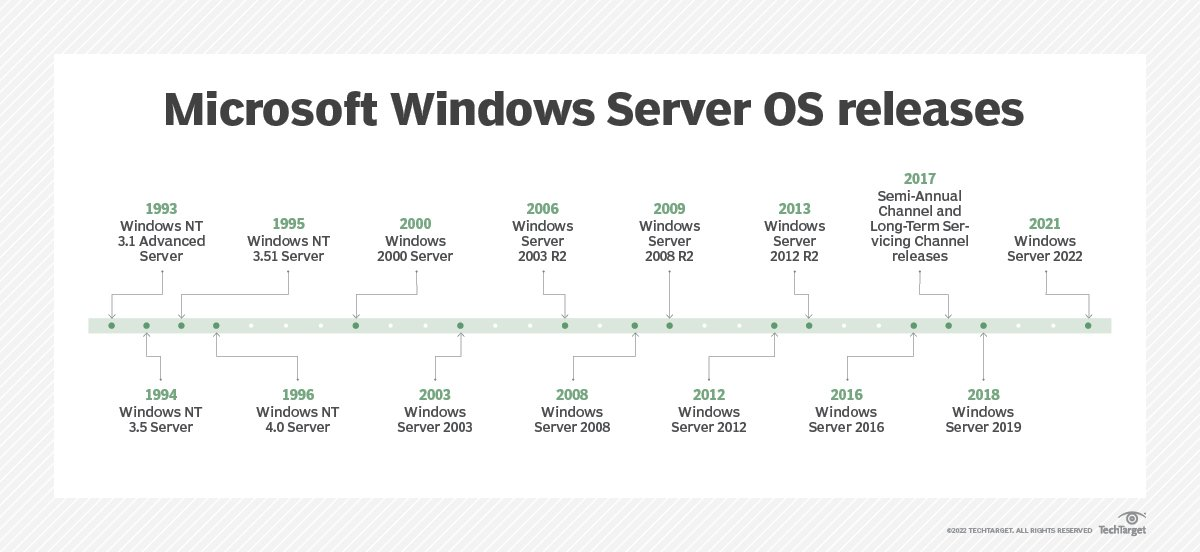
\includegraphics[width=1\textwidth]{timeline.jpeg}
    \caption{ภาพที่ 1 Microsoft Windows Server OS เวอร์ชันวางจำหน่าย (ภาพจาก Tom Walat 2017)}
\end{figure}
\vspace{1cm}

\section{คุณสมบัติที่เป็นจุดเด่น}

\hspace{0cm}\subsection{Azure Edition :}เป็นตัวเลือกการออกใบอนุญาตพิเศษสำหรับ Windows Server 2022 Datacenter ที่ออกแบบมาสำหรับการใช้งานบน Azure โดยเฉพาะ
โดยมีคุณสมบัติเพิ่มเติม เช่น อัปเดตระบบปฏิบัติการโดยไม่ต้องรีบูตเซิร์ฟเวอร์ เหมาะสำหรับ workloads ที่มีความสำคัญสูง เพิ่มประสิทธิภาพการทำงานของ SMB ผ่านเครือข่าย WAN เพิ่มเครือข่ายเสมือนเพิ่มเติมสำหรับ workloads ที่ต้องการการแยกและประสิทธิภาพการจำลองเสมือนที่ดีขึ้นสำหรับ workloads บน Azure \cite{2022:3}

\hspace{1cm}\subsubsection{Storage Replica compression for data transfer :}คือ ฟีเจอร์ใหม่ที่เพิ่มเข้ามาใน Windows Server เพื่อช่วยลดขนาดข้อมูลที่ถูกส่งต่อระหว่างเซิร์ฟเวอร์ต้นทางและเซิร์ฟเวอร์ปลายทาง การบีบอัดนี้จะทำการลดขนาดของข้อมูลที่ถูกส่งผ่านเครือข่ายทำให้ใช้แบนด์วิดธ์น้อยลง และสามารถส่งข้อมูลได้เร็วขึ้น ซึ่งจะช่วยเพิ่มประสิทธิภาพในการส่งข้อมูลและลดการใช้งานของเครือข่าย การใช้งาน Storage Replica compression for data transfer นี้จะช่วยลดเวลาในการซิงโครไนซ์ข้อมูล เช่นในสถานการณ์ฉุกเฉินที่ต้องการความเร่งด่วนในการกู้คืนข้อมูล เป็นต้น

\hspace{1cm}\subsubsection{Support for Azure Stack HCI :}ด้วยเวอร์ชันนี้ สามารถเรียกใช้ Windows Server 2022 Datacenter: Azure Edition ในฐานะ Guest VM ที่รองรับบน Azure Stack HCI เวอร์ชัน 22H2 ด้วย Azure Edition ที่ทำงานบน Azure Stack HCI จะสามารถใช้คุณสมบัติที่มีอยู่ทั้งหมด รวมถึง Hot patch สำหรับ Server Core และ SMB ผ่าน QUIC ที่ศูนย์ข้อมูลและตำแหน่ง Edge ได้

\hspace{1cm}\subsubsection{Azure Auto manage - Hot patch :}Hot patching ซึ่งเป็นส่วนหนึ่งของ Azure Auto manage เป็นวิธีใหม่ในการติดตั้งการอัปเดตบนเครื่องเสมือน (VM) ของ Windows Server Azure Edition ใหม่ ซึ่งไม่จำเป็นต้องรีบูตหลังการติดตั้ง 

\hspace{1cm}\subsubsection{SMB over QUIC :}SMB ผ่าน QUIC อัปเดตโปรโตคอล SMB 3.1.1 เพื่อใช้โปรโตคอล QUIC แทน TCP ใน Windows Server 2022 Datacenter: Azure Edition, Windows 11 และใหม่กว่า และไคลเอนต์บุคคลที่สามหากรองรับ การใช้ SMB บน QUIC ร่วมกับ TLS 1.3 ทำให้ผู้ใช้และแอปพลิเคชันสามารถเข้าถึงข้อมูลจากเซิร์ฟเวอร์ไฟล์ Edge ที่ทำงานอยู่ใน Azure ได้อย่างปลอดภัยและเชื่อถือได้ ผู้ใช้มือถือและโทรคมนาคมไม่จำเป็นต้องใช้ VPN เพื่อเข้าถึงเซิร์ฟเวอร์ไฟล์ผ่าน SMB อีกต่อไปเมื่อใช้ Windows 

\hspace{1cm}\subsubsection{Extended network for Azure :}Azure Extended Network สามารถขยายเครือข่ายย่อยในองค์กรไปยัง Azure เพื่อให้เครื่องเสมือนในองค์กรเก็บที่อยู่ IP ส่วนตัวในองค์กรดั้งเดิมเมื่อย้ายไปยัง Azure 
\clearpage

\hspace{1cm}\subsubsection{Azure hybrid capabilities :}เพิ่มประสิทธิภาพและความคล่องตัวด้วยความสามารถแบบไฮบริดในตัวใน Windows Server 2022 ที่ช่วยให้สามารถขยายศูนย์ข้อมูลไปยัง Azure ได้ง่ายกว่าที่เคย 

\hspace{1cm}\subsubsection{Azure Arc enabled Windows Servers :}เซิร์ฟเวอร์ที่เปิดใช้งาน Azure Arc พร้อม Windows Server 2022 นำเซิร์ฟเวอร์ Windows ภายในองค์กรและมัลติคลาวด์มาสู่ Azure ด้วย Azure Arc ประสบการณ์การจัดการนี้ได้รับการออกแบบมาให้สอดคล้องกับวิธีที่จัดการเครื่องเสมือน Azure ดั้งเดิม เมื่อเครื่องไฮบริดเชื่อมต่อกับ Azure เครื่องนั้นจะกลายเป็นเครื่องที่เชื่อมต่อและถือเป็นทรัพยากรใน Azure 

\vspace{2cm}

\hspace{0cm}\subsection{Security :}เสริมความปลอดภัยให้กับการสื่อสารของเซิร์ฟเวอร์ด้วยการเข้ารหัสลับ SMB AES -256 มาตรฐานอุตสาหกรรมและการควบคุมที่ดีขึ้น รับการป้องกันเชิงป้องกันสำหรับแอสเซทที่ละเอียดอ่อน เช่น ข้อมูลประจำตัวด้วย Credential Guard และการบูตแบบปลอดภัยที่เปิดใช้งานโดยใช้ TPM 2.0 ปกป้องความสมบูรณ์ของระบบจากการโจมตีเฟิร์มแวร์ด้วย Windows Defender System Guard และแยกส่วนที่สำคัญของระบบด้วยการรักษาความปลอดภัยที่ใช้การจำลองเสมือน  

\hspace{1cm}\subsubsection{Secured-core server :}เซิร์ฟเวอร์ที่เปิดใช้งาน Azure Arc พร้อม Windows Server 2022 นำเซิร์ฟเวอร์ Windows ภายในองค์กรและมัลติคลาวด์มาสู่ Azure ด้วย Azure Arc ประสบการณ์การจัดการนี้ได้รับการออกแบบมาให้สอดคล้องกับวิธีที่จัดการเครื่องเสมือน Azure ดั้งเดิม เมื่อเครื่องไฮบริดเชื่อมต่อกับ Azure เครื่องนั้นจะกลายเป็นเครื่องที่เชื่อมต่อและถือเป็นทรัพยากรใน Azure 

\hspace{1cm}\subsubsection{Hardware root-of-trust :}ความน่าเชื่อถือของฮาร์ดแวร์โดยคุณสมบัติต่างๆ เช่นการเข้ารหัสไดรฟ์ด้วย Bit Locke r ชิปประมวลผลการเข้ารหัสที่ปลอดภัย Trusted Platform Module 2.0 (TPM 2.0) มอบการจัดเก็บบนฮาร์ดแวร์ที่ปลอดภัยสำหรับคีย์การเข้ารหัสลับและข้อมูลที่มีความละเอียดอ่อน รวมถึงการวัดความสมบูรณ์ของระบบ TPM 2.0สามารถตรวจสอบได้ว่าเซิร์ฟเวอร์เริ่มต้นด้วยโค้ดที่ถูกต้องตามกฎหมาย และเชื่อถือได้โดยการเรียกใช้โค้ดที่ตามมา ซึ่งเรียกว่าฮาร์ดแวร์รูทออฟทรัสต์ 

\hspace{1cm}\subsubsection{Firmware protection :}การป้องกันเฟิร์มแวร์โดยการดำเนินการด้วยสิทธิพิเศษระดับสูง และมักจะมองไม่เห็นในโซลูชั่นป้องกันไวรัสแบบเดิม ซึ่งทำให้มีการโจมตีด้วยเฟิร์มแวร์เพิ่มมากขึ้น เซิร์ฟเวอร์หลักที่ปลอดภัยจะวัดและตรวจสอบกระบวนการบูตด้วยเทคโนโลยี Dynamic Root of Trust for Measuring (DRTM ) เซิร์ฟเวอร์ Secured-core ยังสามารถแยกการเข้าถึงหน่วยความจำของไดรเวอร์ด้วยการป้องกัน Direct Memory Access (DMA) 
\clearpage

\hspace{1cm}\subsubsection{UEFI secure boot :}การบูตที่ปลอดภัยของ UEFI คือมาตรฐานความปลอดภัยที่ปกป้องเซิร์ฟเวอร์จากรูทคิทที่เป็นอันตราย การบูตแบบปลอดภัยช่วยให้เซิร์ฟเวอร์บู๊ตได้เฉพาะเฟิร์มแวร์และซอฟต์แวร์ที่ผู้ผลิตฮาร์ดแวร์ไว้วางใจเท่านั้น เมื่อเซิร์ฟเวอร์เริ่มทำงาน เฟิร์มแวร์จะตรวจสอบลายเซ็นของส่วนประกอบการบู๊ตแต่ละรายการ รวมถึงไดรเวอร์เฟิร์มแวร์และระบบปฏิบัติการ หากลายเซ็นถูกต้อง เซิร์ฟเวอร์จะบู๊ตและเฟิร์มแวร์จะควบคุมระบบปฏิบัติการ 

\hspace{1cm}\subsubsection{Virtualization-based security (VBS) :}เซิร์ฟเวอร์หลักที่ปลอดภัยรองรับการรักษาความปลอดภัยบนการจำลองเสมือน (VBS) และความถูกต้องของโค้ดบนไฮเปอร์ไวเซอร์ (HVCI) VBSใช้คุณสมบัติการจำลองเสมือนสำหรับฮาร์ดแวร์เพื่อสร้างและแยกพื้นที่หน่วยความจำที่ปลอดภัยออกจากระบบปฏิบัติการปกติ เพื่อป้องกันช่องโหว่ระดับทั้งหมดที่ใช้ในการโจมตีการขุดเหมืองสกุลเงินดิจิทัล VBS ยังอนุญาตให้ใช้ Credential Guard โดยที่ข้อมูลรับรองผู้ใช้และความลับจะถูกจัดเก็บไว้ในคอนเทนเนอร์เสมือนที่ระบบปฏิบัติการไม่สามารถเข้าถึงได้โดยตรง โดย HVCI ใช้ VBS เพื่อเสริมสร้างการบังคับใช้นโยบายความสมบูรณ์ของโค้ด ความสมบูรณ์ของโหมดเคอร์เนลป้องกันไม่ให้ไดรเวอร์โหมดเคอร์เนลหรือไฟล์ระบบที่ไม่ได้ลงนามโหลดลงในหน่วยความจำระบบ มี Kernel Data Protection (KDP) ให้การป้องกันหน่วยความจำแบบอ่านอย่างเดียวของหน่วยความจำเคอร์เนลที่มีข้อมูลที่ไม่สามารถดำเนินการได้ โดยที่เพจหน่วยความจำได้รับการปกป้องโดย Hypervisor KDP ปกป้องโครงสร้างสำคัญในรันไทม์ Windows Defender System Guard จากการถูกดัดแปลง  

\hspace{1cm}\subsubsection{Add Windows Servers :}สามารถเพิ่ม Windows Servers ได้ด้วยกระบวนการที่ง่ายและสะดวกหากต้องการเพิ่ม Windows Servers ใหม่ ให้ไปที่ไอคอน Azure Arc ที่มุมขวาล่างของทาสก์บาร์ แล้วเปิดโปรแกรมการตั้งค่า Azure Arc เพื่อติดตั้งและกำหนดค่า Azure Connected Machine Agent เมื่อติดตั้งแล้วจะสามารถใช้ Azure Connected Machine Agent ได้โดยไม่มีค่าใช้จ่ายเพิ่มเติมสำหรับบัญชี Azure เมื่อเปิดใช้งาน Azure Arc บนเซิร์ฟเวอร์แล้ว สามารถดูข้อมูลสถานะได้ในไอคอนแถบงาน 

\clearpage

\hspace{0cm}\subsection{Application platform :}มีการปรับปรุงแพลตฟอร์มหลายประการสำหรับ Windows Containers รวมถึงความเข้ากันได้ของแอปพลิเคชันและประสบการณ์ Windows Container กับ Kubernetes  คุณสมบัติใหม่บางประการ ได้แก่ : 

\hspace{1cm}\subsubsection{ลดขนาดอิมเมจ Windows Container ลงสูงสุดร้ายละ 40 ส่งผลให้เวลาเริ่มต้นเร็วขึ้นร้อยละ 30 และประสิทธิภาพดีขึ้น}

\hspace{1cm}\subsubsection{แอปพลิเคชันที่จะสามารถใช้ Azure Active Directory กับบัญชี Managed Services Accounts (gMSA) แบบกลุ่มโดยไม่ต้องมีโดเมนเข้าร่วมคอนเทนเนอร์โฮสต์ ขณะนี้ Windows Containers รองรับ Microsoft Distributed Transaction Control (MSDTC) และ Microsoft Message Queuing (MSMQ)}

\hspace{1cm}\subsubsection{สามารถกำหนดบัสธรรมดาให้กับคอนเทนเนอร์ Windows Server ที่แยกกระบวนการได้ แอปพลิเคชันที่ทำงานในคอนเทนเนอร์ที่จำเป็นต้องพูดคุยผ่าน SPI, I2C, GPIO และ UART/COM สามารถทำได้แล้ว }

\hspace{1cm}\subsubsection{เปิดใช้งานการสนับสนุนสำหรับการเร่งด้วยฮาร์ดแวร์ของ DirectX API ในคอนเทนเนอร์ Windows เพื่อรองรับสถานการณ์ต่างๆ เช่น การอนุมานของการเรียนรู้ของเครื่อง (ML) โดยใช้ฮาร์ดแวร์หน่วยประมวลผลกราฟิกในเครื่อง (GPU) }

\hspace{1cm}\subsubsection{Windows Admin Center ได้รับการอัปเดตเพื่อให้ง่ายต่อการบรรจุแอปพลิเคชัน .NET เมื่อแอปพลิเคชันอยู่ในคอนเทนเนอร์ สามารถโฮสต์แอปพลิเคชันนั้นบน Azure Container Registry เพื่อปรับใช้กับบริการ Azure อื่นๆ รวมถึงบริการ Azure Kubernetes }

\hspace{1cm}\subsubsection{รองรับโปรเซสเซอร์ Intel Ice Lake ทำให้ Windows Server 2022 รองรับแอปพลิเคชันที่สำคัญทางธุรกิจและขนาดใหญ่ที่ต้องใช้หน่วยความจำสูงสุด 48 TB และคอร์ลอจิคัล 2,048 คอร์ที่ทำงานบนซ็อกเก็ตจริง 64 ซ็อกเก็ต การประมวลผลที่เป็นความลับด้วย Intel Secured Guard Extension (SGX) บน Intel Ice Lake ช่วยเพิ่มความปลอดภัยของแอปพลิเคชันโดยแยกแอปพลิเคชันออกจากกันด้วยหน่วยความจำที่ได้รับการป้องกัน }

\clearpage



\section{ลักษณะของงานที่เหมาะสม}

\hspace{0cm}\subsubsection{Web Server :}Windows Server รองรับเทคโนโลยีของเว็บที่หลากหลาย รองรับ ASP.NET, PHP, .NET Core และJava ซึ่งเป็นเทคโนโลยีที่ใช้พัฒนาเว็บไซต์และแอปพลิเคชันเว็บที่นิยมมากที่สุด  
มีเครื่องมือจัดการที่ใช้งานง่ายโดย มาพร้อมเครื่องมือจัดการเว็บเซิร์ฟเวอร์ที่ใช้งานง่าย เช่น IIS Manager สามารถติดตั้ง กำหนดค่า และจัดการเว็บเซิร์ฟเวอร์ได้อย่างสะดวก 
มีฟีเจอร์ด้านความปลอดภัยชั้นสูง เช่น HTTPS, HTTP/2 และ Windows Defender Advanced Threat Protection ช่วยให้เว็บไซต์และแอปพลิเคชันให้ปลอดภัยจากภัยคุกคามทางไซเบอร์ 
รองรับการโหลดบาลานซ์ ช่วยให้เว็บไซต์ทำงานได้อย่างราบรื่นและมีประสิทธิภาพ แม้จะมีผู้ใช้เข้าใช้งาน Bandwidth มากก็ตาม 

\hspace{0cm}\subsubsection{File Server :}Windows Server รองรับการเข้าถึงไฟล์แบบพร้อมกันจากหลายอุปกรณ์ ช่วยให้ผู้ใช้สามารถทำงานร่วมกันบนไฟล์เดียวกันได้อย่างสะดวก 
มาพร้อมฟีเจอร์ด้านความปลอดภัยชั้นสูง เช่น NTFS permissions และ BitLocker encryption ช่วยให้ไฟล์ปลอดภัยจากการเข้าถึงโดยไม่ได้รับอนุญาต 
รองรับการสำรองข้อมูล ช่วยให้มั่นใจว่าข้อมูล0yไม่สูญหายในกรณีเกิดอุบัติเหตุ 
มีเครื่องมือจัดการไฟล์ที่ใช้งานง่าย เช่น File Explorer ช่วยให้สามารถจัดการไฟล์ได้อย่างสะดวก 

\hspace{0cm}\subsubsection{Application Server :}Windows Server ทำหน้าที่โฮสต์แอปพลิเคชันบนเซิร์ฟเวอร์ ช่วยให้นักพัฒนาซอฟต์แวร์สามารถ deploy แอปพลิเคชันให้กับผู้ใช้ 
โดยรองรับแอปพลิเคชันแบบ mission-critical ที่ต้องการความเสถียรสูง 
มีความปลอดภัยชั้นสูง เช่น Windows Defender Advanced Threat Protection ช่วยให้แอปพลิเคชันปลอดภัยจากภัยคุกคามทางไซเบอร์ 
รองรับการโหลดบาลานซ์ ช่วยให้แอปพลิเคชันทำงานได้อย่างราบรื่น
มีเครื่องมือช่วยจัดการแอปพลิเคชัน เช่น Server Manager ช่วยให้นักพัฒนาซอฟต์แวร์สามารถ deploy และจัดการแอปพลิเคชันได้อย่างสะดวก

\hspace{0cm}\subsubsection{Mail Server :}Windows Server รองรับ Exchange Server ซึ่งเป็นระบบอีเมลที่ได้รับความนิยม 
มาพร้อมฟีเจอร์ด้านความปลอดภัยชั้นสูง เช่น antivirus and antispam protection ช่วยให้ระบบอีเมลปลอดภัยจากภัยคุกคามทางไซเบอร์ 
รองรับการสำรองข้อมูล ช่วยให้มั่นใจว่าข้อมูลอีเมลจะไม่สูญหาย 
มาพร้อมเครื่องมือจัดการอีเมล เช่น Exchange Management Console ช่วยให้ผู้ดูแลระบบสามารถจัดการระบบอีเมลได้อย่างสะดวก 

\hspace{0cm}\subsubsection{Database Server :}Windows server สามารถรองรับ SQL Server ซึ่งเป็นระบบฐานข้อมูลที่ได้รับความนิยมเป็นอย่างมาก เป็นระบบฐานข้อมูลที่มีประสิทธิภาพ มีความสามารถในการจัดการข้อมูลอย่างมีประสิทธิภาพ และมีความเสถียรที่ดีในการใช้งานร่วมกับ Windows Server 
มาพร้อมฟีเจอร์ด้านความปลอดภัยชั้นสูง เช่น Always On Availability Groups และ Transparent Data Encryption ช่วยให้ระบบฐานข้อมูลปลอดภัยจากภัยคุกคามทางไซเบอร์ 
มีฟีเจอร์การสำรองข้อมูล (Backup) ที่สามารถสำรองข้อมูลของระบบได้อย่างมีประสิทธิภาพและปลอดภัย 

\hspace{0cm}\subsubsection{Backup Server :}สามารถใชเซิร์ฟเวอร์เป็นที่ใช้สำหรับการจัดเก็บข้อมูลสำรอง (Backup) ของระบบและข้อมูลสำคัญขององค์กร เพื่อใช้ในกรณีที่ข้อมูลหลักเสียหาย 
รองรับการสำรองข้อมูลแบบอัตโนมัติ ช่วยให้มั่นใจว่าข้อมูลไม่สูญหาย สามารถตั้งค่าการสำรองข้อมูลให้ทำงานอัตโนมัติตามกำหนดเวลาที่กำหนดได้ เพื่อความสะดวกและป้องกันข้อมูลจากการสูญหายโดยไม่ตั้งใจ 
มีฟีเจอร์ด้านความปลอดภัย เช่น encryption และ compression ที่ช่วยในการป้องกันข้อมูลจากการถูกนำไปใช้โดยได้รับอนุญาตหรือการสูญหาย นอกจากนี้ยังช่วยลดพื้นที่การจัดเก็บข้อมูลและเพิ่มความเร็วในการสำรองข้อมูลรองรับการสำรองข้อมูลไปยังอุปกรณ์ต่างๆ เช่น cloud storage 
มีเครื่องมือจัดการการสำรองข้อมูล เช่น Backup Manager ช่วยให้การสำรองข้อมูลเป็นไปอย่างมีประสิทธิภาพและสะดวกสบาย 

\hspace{0cm}\subsubsection{Remote Desktop Services :} Windows server สำหรับ Remote Desktop Services 
มีความสามารถที่จะอนุญาตให้ผู้ใช้เข้าถึงเดสก์ท็อปเสมือนจริงจากอุปกรณ์ต่างๆ โดยที่เดสก์ท็อปเหล่านั้นจะเป็นเดสก์ท็อปเสมือนจริง 
มีฟีเจอร์ความปลอดภัยเช่น Remote Desktop Gateway และ Network Level Authentication ที่ช่วยให้การเข้าถึงผ่าน RDS มีความปลอดภัย 
รองรับการใช้งานแบบ multi-user ช่วยให้ผู้ใช้หลายคนเข้าถึงเดสก์ท็อปเสมือนจริงพร้อมกันโดยใช้งานบนเซิร์ฟเวอร์เดียวกัน 
มีเครื่องมือจัดการ Remote Desktop Services เช่น Remote Desktop Services Manager ช่วยให้ผู้ดูแลระบบสามารถจัดการและควบคุมการเข้าถึง RDS ได้อย่างมีประสิทธิภาพ   

\hspace{0cm}\subsubsection{Hyper-V Server : }Windows server สำหรับรองรับการรันระบบปฏิบัติการหลายตัวบนเครื่องเดียว  ช่วยให้สามารถรันเซิร์ฟเวอร์หลายตัวในรูปแบบของเครื่องเสมือน (Virtual Machine) บนเครื่องเดียวได้อย่างมีประสิทธิภาพ 
ช่วยให้ประหยัดทรัพยากรฮาร์ดแวร์ การใช้งานเครื่องเสมือนช่วยลดความจำเป็นในการมีเครื่องเซิร์ฟเวอร์หลายตัว 
มีฟีเจอร์ด้านความปลอดภัย เช่น Hyper-V Shielded VMs ซึ่งช่วยป้องกันการเข้าถึงข้อมูลภายในเครื่องเสมือน 
มีเครื่องมือจัดการ Hyper-V Server เช่น Hyper-V Manager เครื่องมือจัดการที่ช่วยให้ผู้ดูแลระบบสามารถจัดการเครื่องเสมือนและการทำงานของเซิร์ฟเวอร์ได้อย่างมีประสิทธิภาพ 

\hspace{0cm}\subsubsection{Disaster Recovery Server :}สามารถกู้คืนระบบและข้อมูลในกรณีฉุกเฉิน สามารถกู้คืนระบบและข้อมูลที่สำคัญในกรณีเกิดเหตุฉุกเฉิน เช่น การเสียหายของฮาร์ดแวร์ ไฟไหม้ หรือการโจมตีจากไวรัส 
ช่วยให้ลด downtime โดยการใช้ Disaster Recovery Server สามารถลดเวลาที่ระบบหยุดทำงาน (downtime) ในกรณีฉุกเฉิน ซึ่งช่วยลดผลกระทบทางธุรกิจ 
มีฟีเจอร์ด้านความปลอดภัย เช่น replication and failover ทำสำเนาข้อมูลและเปลี่ยนเป็นใช้งานได้ทันทีในกรณีฉุกเฉิน 
มีเครื่องมือจัดการ Disaster Recovery Server เช่น Site Recovery Manager จัดการและกู้คืนระบบเป็นไปอย่างมีประสิทธิภาพในกรณีฉุกเฉิน 

\hspace{0cm}\subsubsection{Development Server :}ช่วยให้นักพัฒนาสามารถพัฒนาและทดสอบโปรแกรมหรือแอปพลิเคชันใหม่ได้อย่างมีประสิทธิภาพและปลอดภัย ประหยัดทรัพยากรฮาร์ดแวร์ ลดค่าใช้จ่ายในการจัดซื้อฮาร์ดแวร์เนื่องจากไม่ต้องใช้เครื่องที่ใหญ่และแพงเพื่อการพัฒนา มีฟีเจอร์ด้านความปลอดภัย เช่น debugging and profiling ที่ช่วยในการตรวจสอบและแก้ไขข้อผิดพลาดในโค้ดและยังมีเครื่องมือจัดการ Development Server เช่น Visual Studio ช่วยให้นักพัฒนาสามารถจัดการและพัฒนาโปรแกรมได้อย่างมีประสิทธิภาพ 

\section{ประเภทของอาชีพบุคลากรที่เหมาะสม}

\hspace{0cm}\subsubsection{ผู้ดูแลระบบ (System Administrator)}
เป็นคนที่ทำหน้าที่ในการติดตั้ง กำหนดค่า ดูแลรักษา และแก้ไขปัญหาเกี่ยวกับ Windows Server จำเป็นต้องมีความรู้เกี่ยวกับระบบปฏิบัติการ Windows Server เครือข่าย ฮาร์ดแวร์ และซอฟต์แวร์ต่างๆ มีความรู้ความสามารถในการดูแลรักษาระบบให้มีความปลอดภัย และต้องทำ report performance ของ server ทำแบคอัพ network monitoring ตรวจสอบความผิดปกติที่จะเกิดขึ้นกับระบบได้  ต้องติดตั้ง ฮาร์ดแวร์ ซอฟต์แวร์ application ต่าง ๆ รวมทั้ง patch และปรับแต่งระบบตามความต้องการขององค์กร แก้ไขปัญหาต่างๆที่เกิดขึ้นกับระบบและ support user \cite{job:1}

\hspace{0cm}\subsubsection{วิศวกร DevOps (DevOps Engineer)}ทำหน้าที่ในการพัฒนาและใช้งานระบบอัตโนมัติสำหรับการจัดการ
Windows Server ออกแบบระบบการทดสอบซอฟต์แวร์ให้มีประสิทธิภาพ ตรวจสอบระบบและซอฟต์แวร์ว่าสามารถทำงานได้อย่างมีประสิทธิภาพหรือไม่ 
ออกแบบระบบการทดสอบอัตโนมัติ แก้ไขปัญหาที่เกิดขึ้นกับซอฟต์แวร์ให้ทำงานได้มีประสิทธิภาพมากขึ้น ประสานงานกับแผนกอื่น ๆ ที่เกี่ยวข้องเพื่อออกแบบระบบการทำงานให้ราบรื่นมากขึ้น \cite{job:2}

\hspace{0cm}\subsubsection{นักพัฒนาซอฟต์แวร์ (Software Developer)}ผู้ที่ความเชี่ยวชาญในการออกแบบ การวางแผนพัฒนา เน้นในเรื่องของการเขียนโปรแกรม โดยใช้ภาษาโปรแกรมใดภาษาหนึ่ง รวมไปถึงการบริหารโปรเจกต์และออกแบบฟีเจอร์ต่างๆ ซึ่งขอบเขตงานจะกว้างกว่าการเขียนโปรแกรม โดยอาจมีส่วนร่วมในทั้งโปรเจคมากกว่าดูแลส่วนของชิ้นงาน ลักษณะงานหลัก ๆ ที่ทำจะเป็นการวิเคราะห์ และพัฒนาระบบซอฟต์แวร์ ศึกษากระบวนการ ตลอดจนเทคโนโลยีที่เกี่ยวข้อง ทำการออกแบบกระบวนการในการทำระบบซอฟต์แวร์ให้เป็นมาตรฐาน ทำหน้าที่พัฒนาแอปพลิเคชันที่ทำงานบน Windows Serve ทำการทดสอบและตรวจสอบความถูกต้องของกระบวนการให้เป็นไปตามความต้องการ ทำการประเมินผลการทำงานของแต่ละขั้นตอนในกระบวนการ พร้อมประเมินผลความเสี่ยง สนับสนุนการพัฒนาซอฟต์แวร์ระบบใหญ่ให้มีคุณภาพสูง \cite{job:3}
\clearpage
\hspace{0cm}\subsubsection{ผู้เชี่ยวชาญด้านความปลอดภัย}มีความเชี่ยวชาญเฉพาะด้านในสายงานไอที ทำหน้าที่ดูแลความมั่นคงและปลอดภัยทางไซเบอร์ รักษาความปลอดภัยของ Server ไม่ว่าจะเป็นการจัดการระบบ ดูแลตรวจสอบ การประเมินความเสี่ยง วิเคราะห์ข้อมูล และการเฝ้าระวังการถูกขโมยข้อมูล เพื่อให้บริษัทหรือองค์กรสามารถป้องกันข้อมูลเอาไว้ได้อย่างมีประสิทธิภาพ \cite{job:4}

\hspace{0cm}\subsubsection{นักวิเคราะห์ข้อมูล}ทำหน้าที่นำข้อมูลจากหลายแหล่งข้อมูลที่รวบรวมไว้ในรูปแบบ Structured Data แล้วโดยใช้ Data Analysis Tool เพื่อสรุปเชิงลึก หา Business Insight หาแนวโน้ม ช่วยธุรกิจในการตัดสินใจหาทางเลือก กำหนดกลยุทธได้ เช่น การลงทุน การลดต้นทุน ราคาขาย การรับพนักงาน การวางแผนการผลิต เป็นต้น เพื่อช่วยสร้างข้อได้เปรียบทางธุรกิจ ซึ่งจำเป็นที่ต้องมีทักษะด้านคณิตศาสตร์ และตัวเลข เข้าใจเรื่องสถิติ มีประสบการณ์ในการสรุปผล เช่น Excel, Power BI เข้าใจฐานข้อมูล เช่น SQL Server, Oracle และ SAPเข้าใจเรื่องสคริปต์และเว็บไซต์ เช่น json, xml, java script, html5 กระบวนการ ETL และการใช้เครื่องมืออย่าง SSIS, Power Query เป็นต้น \cite{job:5}
% การเขียนเอกสารอ้างอิง ให้ใช้รูปแบบ APA7 
% ลักษณะของการเขียนนี้ เป็นแบบ bibtex หากใช้รูปแบบอื่น
% ให้ปรับเป็นแบบ APA7 
%
% หนังสือทั่วไป ให้ใช้รูปแบบ โดยชื่อเรื่องต้องเป็นตัวเอียง ผู้แต่ง 1 - 20 คน ให้ใส่ชื่อทุกคน
%
% ผู้แต่ง. (ปีที่พิมพ์). \textit{ชื่อเรื่อง} (ครั้งที่พิมพ์ พิมพ์ครั้งที่ 2 เป็นต้นไป). สำนักพิมพ์.
%
% เช่น ภาสกร เนตรทิพย์วัลย์, พรพรรณ ภูสาหัส, และวิถี ธุระธรรม. (2565). \textit{การตรวจร่างกาย} (พิมพ์ครั้งที่ 2). พิมพ์ดีการพิมพ์.
% หรือ Kee, J. L., Marshall, S. M., \& Forrester, M. C. (2021). \textit{Clinical calculations} (9th ed.). Elsevier.
%
% ปล. ถ้าไม่ปรากฏปีที่พิมพ์ให้ใส่ (ม.ป.ป.) สำหรับภาษาไทย และ (n.d.) สำหรับภาษาอังกฤษ
%
% วารสารงานวิจัย ให้ใช้รูปแบบดังนี้
%
% ชื่อผู้เขียนบทความ. (ปีที่พิมพ์). ชื่อบทความ. \textit{ชื่อวารสาร}, \textit{เลขฉบับที่ หรือ Volume}(ฉบับที่ หรือ issue), หน้าแรก-หน้าสุดท้าย.
%
% เช่น บุศรา ชัยทัศน์. (2559). การดูแลผู้ป่วยโรงมะเร็งลำไส้ใหญ่. \textit{วารสารพยาบาลสภากาชาดไทย}, \textit{9}(1),19-33.
%หรือ Plows, J. F., Stanley, J. L., \& Vickers, M. H. (2018). The pathophysiology of gestational diabetes metllitus. \textit{International journal of molecular sciences}, \textit{19}(11), 3342.
% https:/doi.org/10.3390/ijms19113342 [arXiv:2210.07273 [astro-ph.HE]]
%
% ปล. ต้องใส่เลข doi ในรูปแบบลิงค์ https และอ้างอิง arXiv ใน [...] ด้วย ถ้ามี
%
% ดูเพิ่มเติมจาก https://tinyurl.com/4p6c5mf5

\begin{thebibliography}{99}
%\addcontentsline{toc}{chapter}{\numberline{}\textbf{บรรณานุกรม}}

\bibitem{ประวัติความเป็นมา:1}
bestinternet.co.th (2561). \textbf{Windows Server คืออะไร} เข้าถึงเมื่อ 16 กุมภาพันธ์. เข้าถึงได้จาก  https://www.bestinternet.co.th/single\_blog.php?id=94

\bibitem{ประวัติความเป็นมา:2}
addin.co.th (2565). \textbf{Windows Server คืออะไร มีกี่ประเภท กี่แบบ กี่เวอร์ชั่น และมีวิธีเลือกซื้อมาใช้งานอย่างไรบ้าง} เข้าถึงเมื่อ 16 กุมภาพันธ์. เข้าถึงได้จาก https://addin.co.th/blog/windows-server/

\bibitem{ประวัติความเป็นมา:Windows Server}
techtarget.com (2560). \textbf{Microsoft Windows Server OS (operating system)} เข้าถึงเมื่อ 16 กุมภาพันธ์. เข้าถึงได้จาก https://www.techtarget.com/searchwindowsserver/definition/Microsoft-Windows-Server-OS-operating-system

\bibitem{ประวัติความเป็นมา:2019}
blognone.com (2561). \textbf{Windows Server 2019 ออกตัวจริงแล้ว} เข้าถึงเมื่อ 16 กุมภาพันธ์. เข้าถึงได้จาก https://www.blognone.com/node/105700

\bibitem{2022:1}
learn.microsoft.com (2566). \textbf{What's new in Windows Server 2022} เข้าถึงเมื่อ 16 กุมภาพันธ์. เข้าถึงได้จาก
https://learn.microsoft.com/th-th/windows-server/get-started/whats-new-in-windows-server-2022

\bibitem{2022:2}
blognone.com (2564). \textbf{Windows Server 2022 ยกระดับความปลอดภัย, เน้นทำงานไฮบริด, อิมเมจขนาดเล็กลง} เข้าถึงเมื่อ 16 กุมภาพันธ์. เข้าถึงได้จาก
https://www.blognone.com/node/121489

\bibitem{2022:3}
learn.microsoft.com (2566). \textbf{What is Azure Edition for Windows Server?} เข้าถึงเมื่อ 16 กุมภาพันธ์. เข้าถึงได้จาก
https://learn.microsoft.com/en-us/windows-server/get-started/azure-edition 

\bibitem{job:1}
th.jobsdb.com (2566). \textbf{System Administrator ผู้ดูแลและจัดการระบบคอมพิวเตอร์ที่ทุกบริษัทควรต้องมี} เข้าถึงเมื่อ 16 กุมภาพันธ์. เข้าถึงได้จาก
https://th.jobsdb.com/th/career-advice/article/system-administrator

\clearpage
\bibitem{job:2}
th.jobsdb.com (2566). \textbf{วิศวกร DevOps เป็นผู้ที่เชื่อมขั้นตอนการพัฒนาซอฟต์แวร์ และนำขึ้นไปทดลองใช้ พร้อมสร้างระบบโครงสร้างพื้นฐานของซอฟต์แวร์ ให้ใช้งานได้อย่างราบรื่น} เข้าถึงเมื่อ 16 กุมภาพันธ์. เข้าถึงได้จาก
https://th.jobsdb.com/th/career-advice/role/devops-engineer


\bibitem{job:3}
th.jobsdb.com (2566). \textbf{เจาะลึก นักพัฒนาซอฟต์แวร์ (Software Developer) อาชีพในฝันของคนรุ่นใหม่} เข้าถึงเมื่อ 16 กุมภาพันธ์. เข้าถึงได้จาก
https://th.jobsdb.com/th/career-advice/article/software-developer

\bibitem{job:4}
bu.ac.th (2564). \textbf{เจาะลึกอาชีพผู้เชี่ยวชาญความปลอดภัยไซเบอร์ คณะเทคโนโลยีสารสนเทศและนวัตกรรม} เข้าถึงเมื่อ 16 กุมภาพันธ์. เข้าถึงได้จาก
https://www.bu.ac.th/th/featured-stories/636


\bibitem{job:5}
9experttraining.com (ม.ป.ป.). \textbf{รู้จักกับ Data Analyst และทักษะที่ต้องรู้} เข้าถึงเมื่อ 16 กุมภาพันธ์. เข้าถึงได้จาก
https://www.9experttraining.com/articles/data-analyst-\%E0\%B8\%84\%E0\%B8\%B7\%E0\%B8\%AD\%E0\%B9\%83\%E0\%B8\%84\%E0\%B8\%A3
\end{thebibliography}

\end{document}

